\documentclass[8pt,aspectratio=169]{beamer}
\usepackage[utf8]{inputenc}
\usepackage{graphicx}
\usepackage{amsmath,amssymb}
\usepackage{listings}
\usepackage{xcolor}
\usepackage{tikz}
\usepackage{tcolorbox}

\usetheme{Madrid}
\usecolortheme{seahorse}
\setbeamertemplate{navigation symbols}{}
\setbeamertemplate{footline}[frame number]

\definecolor{darkblue}{RGB}{0,51,102}
\definecolor{lightblue}{RGB}{173,216,230}
\definecolor{codegreen}{RGB}{0,128,0}
\definecolor{codegray}{RGB}{150,150,150}
\definecolor{backcolor}{RGB}{245,245,245}

\lstset{
    backgroundcolor=\color{backcolor},
    basicstyle=\ttfamily\tiny,
    breaklines=true,
    language=Python
}

\newcommand{\given}{\mid}
\newcommand{\highlight}[1]{\textcolor{red}{\textbf{#1}}}
\newcommand{\eqbox}[1]{\begin{tcolorbox}[colback=blue!5!white,colframe=blue!75!black]#1\end{tcolorbox}}

\title[Week 4: Seq2Seq]{Natural Language Processing}
\subtitle{Week 4: The Compression Journey}
\institute{From Meaning to Numbers and Back Again}
\author{}
\date{}

\begin{document}

\begin{frame}
    \titlepage
\end{frame}

\begin{frame}{Learning Objectives}
    \textbf{By the end of this lecture, you will understand:}
    \begin{enumerate}
        \item Why we need numbers to represent words (from first principles)
        \item How compression creates an information bottleneck
        \item What ``context'' and ``hidden state'' actually mean
        \item How attention solves the compression problem
        \item Why this matters for all modern NLP
    \end{enumerate}

    \vspace{1em}
    \textbf{Prerequisites from Week 3:}
    \begin{itemize}
        \item Basic understanding that neural networks process numbers
        \item Concept of sequential processing (RNN idea)
        \item Backpropagation intuition
    \end{itemize}
\end{frame}

\begin{frame}{Table of Contents}
    \tableofcontents
\end{frame}

\section{Act 1: The Compression Challenge}

\begin{frame}[t]{The Core Problem: Computers Don't Understand Words}
    \textbf{Start with the fundamental challenge:}

    \vspace{0.5em}
    You want to translate: ``The black cat sat on the mat'' $\rightarrow$ French

    \vspace{0.5em}
    \textbf{The Computer's Dilemma:}
    \begin{itemize}
        \item Computer sees: \texttt{['T', 'h', 'e', ' ', 'b', 'l', 'a', ...]}
        \item These are just character codes (bytes)
        \item \highlight{No meaning, no relationships, no structure}
    \end{itemize}

    \vspace{0.5em}
    \begin{columns}[T]
        \column{0.5\textwidth}
        \textbf{What the computer sees:}
        \begin{itemize}
            \item ``cat'' = [99, 97, 116]
            \item ``dog'' = [100, 111, 103]
            \item ``sat'' = [115, 97, 116]
        \end{itemize}

        \column{0.5\textwidth}
        \textbf{Problem:}
        \begin{itemize}
            \item ``cat'' and ``sat'' share [97, 116]
            \item Does that mean they're similar?
            \item \textcolor{red}{No! Character overlap $\neq$ meaning}
        \end{itemize}
    \end{columns}

    \vspace{1em}
    \textbf{Key Question:} How do we give computers a ``numerical understanding'' of word meaning?
\end{frame}

\begin{frame}[t]{From Words to Numbers: The Embedding Idea}
    \textbf{The solution: Represent each word as a vector of numbers}

    \vspace{0.5em}
    \textbf{Build intuition with simple example:}

    Imagine describing animals with just 3 properties:
    \begin{itemize}
        \item Size (0=tiny, 1=huge)
        \item Cuteness (0=scary, 1=adorable)
        \item Speed (0=slow, 1=fast)
    \end{itemize}

    \vspace{0.5em}
    \begin{center}
    \begin{tabular}{|l|c|c|c|}
        \hline
        \textbf{Word} & \textbf{Size} & \textbf{Cute} & \textbf{Speed} \\
        \hline
        cat & 0.3 & 0.9 & 0.6 \\
        dog & 0.5 & 0.8 & 0.5 \\
        mouse & 0.1 & 0.7 & 0.8 \\
        elephant & 0.95 & 0.4 & 0.2 \\
        \hline
    \end{tabular}
    \end{center}

    \vspace{0.5em}
    Now computers can compute:
    \begin{itemize}
        \item Similarity: cat $\approx$ dog (vectors are close)
        \item Difference: cat $\neq$ elephant (vectors are far)
        \item \highlight{This is called a ``word embedding''}
    \end{itemize}

    \vspace{0.5em}
    \textbf{Reality:} We use 100-300 dimensions (not just 3), learned from data
\end{frame}

\begin{frame}[t]{What is a ``Hidden State''? Building Intuition}
    \textbf{Now we have numbers for words. Next problem: Understanding sentences}

    \vspace{0.5em}
    \textbf{Human analogy - Reading comprehension:}

    As you read ``The black cat sat on the mat'':
    \begin{enumerate}
        \item After ``The'' $\rightarrow$ You know: article, something coming
        \item After ``The black'' $\rightarrow$ You know: a dark-colored thing
        \item After ``The black cat'' $\rightarrow$ You know: a specific animal
        \item After full sentence $\rightarrow$ You know: complete scene
    \end{enumerate}

    \vspace{0.5em}
    \textbf{Your ``understanding'' evolves as you read!}

    \vspace{1em}
    \textbf{Neural network equivalent:}
    \begin{itemize}
        \item Network maintains a vector that represents ``current understanding''
        \item This vector updates with each new word
        \item \highlight{This evolving vector is called the ``hidden state''}
        \item Final hidden state = complete understanding of sentence
    \end{itemize}

    \vspace{0.5em}
    \textbf{Technical name:} When we update understanding word-by-word, we call this a ``Recurrent Neural Network'' (RNN from Week 3)
\end{frame}

\begin{frame}[t]{The Compression Problem Emerges}
    \textbf{Now the real challenge appears:}

    \vspace{0.5em}
    We need to translate: ``The black cat sat on the mat'' $\rightarrow$ ``Le chat noir s'est assis sur le tapis''

    \vspace{0.5em}
    \textbf{Two-stage process (like human translation):}

    \begin{center}
    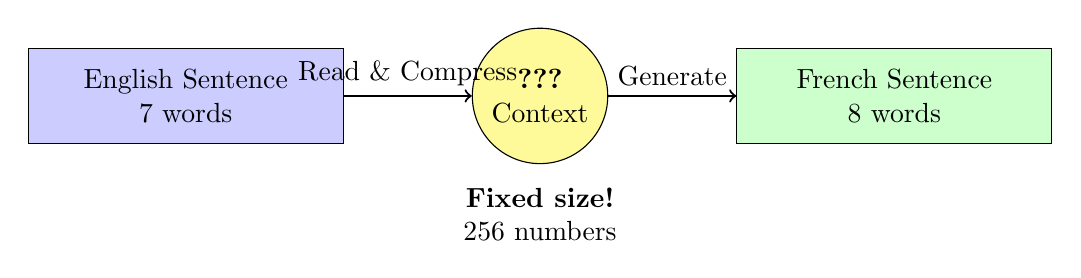
\begin{tikzpicture}[scale=0.9]
        \node[draw, rectangle, minimum width=4cm, minimum height=1.2cm, fill=blue!20, align=center] (input) at (0,0) {English Sentence\\7 words};

        \node[draw, circle, fill=yellow!40, minimum size=1.5cm, align=center] (compressed) at (5,0) {\textbf{???}\\Context};

        \node[draw, rectangle, minimum width=4cm, minimum height=1.2cm, fill=green!20, align=center] (output) at (10,0) {French Sentence\\8 words};

        \draw[->, thick] (input) -- (compressed) node[midway, above] {Read \& Compress};
        \draw[->, thick] (compressed) -- (output) node[midway, above] {Generate};

        \node[below of=compressed, node distance=1.5cm, align=center] {\textbf{Fixed size!}\\256 numbers};
    \end{tikzpicture}
    \end{center}

    \vspace{0.5em}
    \textbf{The bottleneck:}
    \begin{itemize}
        \item 7 words of meaning $\rightarrow$ compressed to 256 numbers
        \item Then generate 8 words from just those 256 numbers
        \item \highlight{Can 256 numbers hold all the information?}
    \end{itemize}

    \vspace{0.5em}
    \textbf{Key Question:} What happens with longer sentences? 100 words $\rightarrow$ still 256 numbers?
\end{frame}

\begin{frame}[t]{Quantifying the Compression Problem}
    \textbf{Let's calculate how much compression we're doing:}

    \vspace{0.5em}
    \textbf{Information content (rough estimate):}
    \begin{itemize}
        \item Each word embedding: 100 dimensions (numbers)
        \item 7-word sentence: $7 \times 100 = 700$ numbers of information
        \item Context vector: \textbf{only 256 numbers}
        \item \highlight{Compression ratio: 700:256 $\approx$ 2.7:1}
    \end{itemize}

    \vspace{0.5em}
    \textbf{What about longer sentences?}

    \begin{center}
    \begin{tabular}{|l|c|c|c|c|}
        \hline
        \textbf{Length} & \textbf{Input Dims} & \textbf{Context Dims} & \textbf{Ratio} & \textbf{Quality} \\
        \hline
        5 words & 500 & 256 & 2:1 & Good \\
        20 words & 2000 & 256 & 8:1 & Mediocre \\
        50 words & 5000 & 256 & 20:1 & Poor \\
        100 words & 10000 & 256 & 40:1 & Very Poor \\
        \hline
    \end{tabular}
    \end{center}

    \vspace{0.5em}
    \begin{tcolorbox}[colback=red!10!white,colframe=red!75!black]
    \textbf{The Information Bottleneck:} Longer sentences lose more information!

    Like trying to fit a whole book into a single paragraph - something must be lost.
    \end{tcolorbox}

    \vspace{0.5em}
    \textbf{Next question:} Can we avoid this bottleneck? (Spoiler: Yes, with attention!)
\end{frame}

\section{Act 2: The Encoder-Decoder Solution (And Its Limits)}

\begin{frame}[t]{The Two-Network Architecture}
    \textbf{The key insight: Separate ``reading'' from ``writing''}

    \vspace{0.5em}
    \textbf{Why two networks? Build from human behavior:}

    When YOU translate:
    \begin{enumerate}
        \item \textbf{Phase 1 (Reading):} Read and understand the English sentence
        \begin{itemize}
            \item Process word-by-word
            \item Build complete understanding
            \item Store meaning in your memory
        \end{itemize}
        \item \textbf{Phase 2 (Writing):} Generate the French translation
        \begin{itemize}
            \item Start from your understanding
            \item Generate word-by-word in French
            \item Use grammar and vocabulary of target language
        \end{itemize}
    \end{enumerate}

    \vspace{0.5em}
    \textbf{Neural equivalent:}
    \begin{itemize}
        \item \textbf{Encoder network:} Reads input, builds ``hidden state'' (understanding)
        \item \textbf{Context vector:} Final hidden state (compressed meaning)
        \item \textbf{Decoder network:} Generates output from context
    \end{itemize}

    \vspace{0.5em}
    \textbf{Technical names you now understand:}
    \begin{itemize}
        \item ``Sequence-to-Sequence'' (Seq2Seq) = this two-network setup
        \item ``Encoder-Decoder architecture'' = same thing
    \end{itemize}
\end{frame}

\begin{frame}[fragile,t]{Encoder: Building Understanding Step-by-Step}
    \textbf{Concrete example: Encoding ``The cat sat''}

    \vspace{0.5em}
    \begin{columns}[T]
        \column{0.55\textwidth}
        \textbf{Step-by-step processing:}

        \textbf{Step 1: Read ``The''}
        \begin{itemize}
            \item Convert to embedding: [0.2, 0.5, -0.1, ...] (100d)
            \item Initial understanding: $h_0$ = [0, 0, 0, ...] (256d)
            \item Update: $h_1$ = RNN(``The'', $h_0$)
            \item New understanding: [0.1, -0.05, 0.03, ...] (256d)
        \end{itemize}

        \textbf{Step 2: Read ``cat''}
        \begin{itemize}
            \item Embedding: [0.7, -0.3, 0.4, ...] (100d)
            \item Previous understanding: $h_1$
            \item Update: $h_2$ = RNN(``cat'', $h_1$)
            \item New understanding: [0.3, 0.2, -0.1, ...] (256d)
        \end{itemize}

        \textbf{Step 3: Read ``sat''}
        \begin{itemize}
            \item Embedding: [-0.2, 0.6, 0.1, ...]
            \item Update: $h_3$ = RNN(``sat'', $h_2$)
            \item \highlight{Final understanding: $h_3$ = context vector}
        \end{itemize}

        \column{0.43\textwidth}
        \begin{center}
        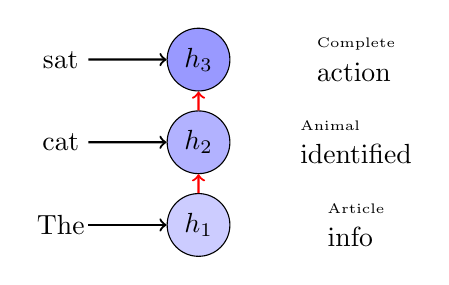
\begin{tikzpicture}[scale=0.7]
            \node at (0,0) {The};
            \node at (0,1.5) {cat};
            \node at (0,3) {sat};

            \node[draw, circle, fill=blue!20] (h1) at (2.5,0) {$h_1$};
            \node[draw, circle, fill=blue!30] (h2) at (2.5,1.5) {$h_2$};
            \node[draw, circle, fill=blue!40] (h3) at (2.5,3) {$h_3$};

            \draw[->, thick] (0.5,0) -- (h1);
            \draw[->, thick] (0.5,1.5) -- (h2);
            \draw[->, thick] (0.5,3) -- (h3);

            \draw[->, thick, red] (h1) -- (h2);
            \draw[->, thick, red] (h2) -- (h3);

            \node[right of=h1, node distance=2cm, align=left] {\tiny Article\\info};
            \node[right of=h2, node distance=2cm, align=left] {\tiny Animal\\identified};
            \node[right of=h3, node distance=2cm, align=left] {\tiny Complete\\action};
        \end{tikzpicture}
        \end{center}

        \vspace{1em}
        \textbf{Key insight:}
        \begin{itemize}
            \item Each $h_t$ = accumulated understanding
            \item Always 256 dimensions
            \item Final $h_3$ goes to decoder
        \end{itemize}
    \end{columns}
\end{frame}

\begin{frame}[fragile,t]{Decoder: Generating from Understanding}
    \textbf{Now generate French from the context vector}

    \vspace{0.5em}
    \begin{columns}[T]
        \column{0.55\textwidth}
        \textbf{Generation process:}

        \textbf{Step 0: Start}
        \begin{itemize}
            \item Input: <START> token
            \item Context: $c = h_3$ from encoder (256d)
            \item Generate: $s_0$ = RNN(<START>, $c$)
            \item Predict probabilities: P(``Le'') = 0.6, P(``Un'') = 0.3, ...
            \item \highlight{Choose ``Le''}
        \end{itemize}

        \textbf{Step 1: Continue}
        \begin{itemize}
            \item Input: ``Le'' (what we just generated)
            \item Context: still $c$ (same context!)
            \item Generate: $s_1$ = RNN(``Le'', $s_0$, $c$)
            \item Predict: P(``chat'') = 0.7, P(``chien'') = 0.2, ...
            \item \highlight{Choose ``chat''}
        \end{itemize}

        \textbf{Step 2: Continue until <END>}
        \begin{itemize}
            \item Input: ``chat''
            \item Generate: $s_2$ = RNN(``chat'', $s_1$, $c$)
            \item Keep going until model outputs <END>
        \end{itemize}

        \column{0.43\textwidth}
        \begin{center}
        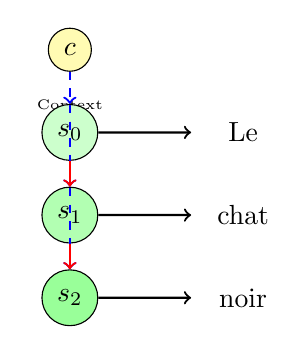
\begin{tikzpicture}[scale=0.7]
            \node[draw, circle, fill=yellow!30] (context) at (0,4) {$c$};
            \node[below of=context, node distance=0.7cm] {\tiny Context};

            \node[draw, circle, fill=green!20] (s0) at (0,2.5) {$s_0$};
            \node[draw, circle, fill=green!30] (s1) at (0,1) {$s_1$};
            \node[draw, circle, fill=green!40] (s2) at (0,-0.5) {$s_2$};

            \node[right of=s0, node distance=2.2cm] {Le};
            \node[right of=s1, node distance=2.2cm] {chat};
            \node[right of=s2, node distance=2.2cm] {noir};

            \draw[->, thick, blue, dashed] (context) -- (s0);
            \draw[->, thick, blue, dashed] (context) -- (s1);
            \draw[->, thick, blue, dashed] (context) -- (s2);

            \draw[->, thick, red] (s0) -- (s1);
            \draw[->, thick, red] (s1) -- (s2);

            \draw[->, thick] (s0) -- (2.2,2.5);
            \draw[->, thick] (s1) -- (2.2,1);
            \draw[->, thick] (s2) -- (2.2,-0.5);
        \end{tikzpicture}
        \end{center}

        \vspace{0.5em}
        \textbf{Key observations:}
        \begin{itemize}
            \item Context $c$ used at every step
            \item Previous word fed back in
            \item Generate one word at a time
            \item Stop when <END> predicted
        \end{itemize}
    \end{columns}
\end{frame}

\begin{frame}[fragile,t]{What Does ``Dot Product Similarity'' Mean?}
    \textbf{Building geometric intuition from scratch}

    \vspace{0.5em}
    \textbf{Start with 2D vectors (easy to visualize):}

    \begin{columns}[T]
        \column{0.5\textwidth}
        Two vectors in 2D space:
        \begin{itemize}
            \item $\vec{a} = [3, 4]$
            \item $\vec{b} = [4, 3]$
        \end{itemize}

        \vspace{0.5em}
        \textbf{Dot product calculation:}
        \begin{align*}
            \vec{a} \cdot \vec{b} &= (3 \times 4) + (4 \times 3)\\
            &= 12 + 12 = 24
        \end{align*}

        \vspace{0.5em}
        \textbf{Geometric meaning:}
        \begin{itemize}
            \item Vectors point similar direction $\rightarrow$ Large positive value
            \item Perpendicular $\rightarrow$ Zero
            \item Opposite directions $\rightarrow$ Large negative value
        \end{itemize}

        \column{0.5\textwidth}
        \begin{center}
        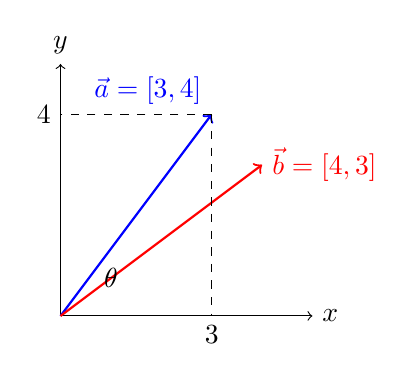
\begin{tikzpicture}[scale=0.8]
            \draw[->] (0,0) -- (4,0) node[right] {$x$};
            \draw[->] (0,0) -- (0,4) node[above] {$y$};

            \draw[->, thick, blue] (0,0) -- (2.4,3.2) node[above left] {$\vec{a}=[3,4]$};
            \draw[->, thick, red] (0,0) -- (3.2,2.4) node[right] {$\vec{b}=[4,3]$};

            \draw[dashed] (2.4,3.2) -- (2.4,0) node[below] {3};
            \draw[dashed] (2.4,3.2) -- (0,3.2) node[left] {4};

            \node at (0.8,0.6) {$\theta$};
        \end{tikzpicture}

        \vspace{0.5em}
        Small angle $\theta$ = similar direction
        \end{center}
    \end{columns}

    \vspace{0.5em}
    \textbf{Why this matters for attention:}
    \begin{itemize}
        \item Decoder state: $h_t^{dec} = [0.5, -0.2, 0.8, ...]$ (256d)
        \item Encoder state: $h_i^{enc} = [0.6, -0.1, 0.7, ...]$ (256d)
        \item Dot product $h_t^{dec} \cdot h_i^{enc}$ = how aligned they are
        \item \highlight{High value = encoder state $i$ is relevant for decoder step $t$}
    \end{itemize}
\end{frame}

\begin{frame}[t]{The Bottleneck Returns: Experimental Evidence}
    \textbf{Does the encoder-decoder actually work well?}

    \vspace{0.5em}
    \textbf{Experimental results (Bahdanau et al., 2014):}

    \begin{center}
    \begin{tabular}{|l|c|c|c|}
        \hline
        \textbf{Sentence Length} & \textbf{Compression} & \textbf{BLEU Score} & \textbf{Quality} \\
        \hline
        5-10 words & 2:1 & 31.5 & Good \\
        10-20 words & 5:1 & 26.3 & Acceptable \\
        20-30 words & 10:1 & 18.7 & Poor \\
        30-40 words & 15:1 & 12.4 & Very Poor \\
        40+ words & 20:1 & 8.1 & Terrible \\
        \hline
    \end{tabular}
    \end{center}

    \vspace{0.5em}
    \textbf{What gets lost in long sentences?}

    \small
    \textit{Input:} ``The International Conference on Machine Learning, which is one of the premier venues for presenting machine learning research and attracts submissions from researchers around the world, accepted our paper.''

    \textit{Translation loses:} ``International'', ``premier venues'', ``around the world'' details

    \textit{Keeps only:} General topic (ML conference), sentiment (positive), main fact (paper accepted)

    \vspace{0.5em}
    \begin{tcolorbox}[colback=red!10!white,colframe=red!75!black]
    \textbf{Problem:} Single context vector is the bottleneck - longer sentences lose 70+ percent quality!
    \end{tcolorbox}
\end{frame}

\section{Act 3: The Attention Revolution}

\begin{frame}[t]{The Human Insight: Selective Focus}
    \textbf{How do YOU actually translate?}

    \vspace{0.5em}
    Translating: ``The black cat sat on the mat'' $\rightarrow$ ``Le chat noir s'est assis sur le tapis''

    \vspace{0.5em}
    \textbf{Honest introspection:}

    \begin{itemize}
        \item Writing ``Le'' $\rightarrow$ You look back at ``The''
        \item Writing ``chat'' $\rightarrow$ You look back at ``cat''
        \item Writing ``noir'' $\rightarrow$ You look back at ``black''
        \item Writing ``s'est assis'' $\rightarrow$ You look back at ``sat''
    \end{itemize}

    \vspace{0.5em}
    \textbf{Key observation:}
    \begin{itemize}
        \item You DON'T compress everything into one memory
        \item You keep the original English visible
        \item You \highlight{selectively attend} to relevant words
        \item Different output words need different input words
    \end{itemize}

    \vspace{1em}
    \begin{tcolorbox}[colback=green!10!white,colframe=green!75!black]
    \textbf{Brilliant idea (Bahdanau et al., 2015):} Let the decoder look back at ALL encoder states, not just the final one!
    \end{tcolorbox}
\end{frame}

\begin{frame}[t]{Attention Mechanism: From Intuition to Math}
    \textbf{The attention solution in 3 steps:}

    \vspace{0.5em}
    \textbf{Step 1: Keep all encoder states (not just last one)}
    \begin{itemize}
        \item After encoding ``The cat sat'': Keep $[h_1^{enc}, h_2^{enc}, h_3^{enc}]$
        \item Each $h_i^{enc}$ represents understanding up to word $i$
        \item \highlight{No compression yet - all information preserved!}
    \end{itemize}

    \vspace{0.5em}
    \textbf{Step 2: Compute relevance scores (the ``attention'' scores)}
    \begin{itemize}
        \item For each decoder step $t$, compute how relevant each encoder state is
        \item Use dot product (geometric similarity we learned earlier):
        \item $score_i = h_t^{dec} \cdot h_i^{enc}$
        \item High score = state $i$ is relevant for current output
    \end{itemize}

    \vspace{0.5em}
    \textbf{Step 3: Weighted combination (dynamic context)}
    \begin{itemize}
        \item Convert scores to probabilities (softmax): $\alpha_i = \frac{\exp(score_i)}{\sum_j \exp(score_j)}$
        \item Weighted average: $context_t = \sum_i \alpha_i \cdot h_i^{enc}$
        \item \highlight{Different context for each decoder step!}
    \end{itemize}

    \vspace{0.5em}
    \textbf{Technical name:} These $\alpha_i$ weights are called ``attention weights'' (where the model is ``paying attention'')
\end{frame}

\begin{frame}[t]{Attention: Concrete Numerical Example}
    \textbf{Let's calculate attention for generating ``chat''}

    \vspace{0.5em}
    \textbf{Setup:}
    \begin{itemize}
        \item Encoder states from ``The cat sat'': $h_1, h_2, h_3$ (each 256d)
        \item Decoder state when generating 2nd word: $s_1$ (256d)
    \end{itemize}

    \vspace{0.5em}
    \begin{columns}[T]
        \column{0.6\textwidth}
        \textbf{Step 1: Compute relevance scores}

        \small
        \begin{align*}
            score_1 &= s_1 \cdot h_1^{enc} &&= 0.08 &&\text{(``The'')}\\
            score_2 &= s_1 \cdot h_2^{enc} &&= 0.92 &&\text{(``cat'')}\\
            score_3 &= s_1 \cdot h_3^{enc} &&= 0.15 &&\text{(``sat'')}
        \end{align*}

        \vspace{0.5em}
        \textbf{Step 2: Softmax to get weights}

        \begin{align*}
            \alpha_1 &= \frac{e^{0.08}}{e^{0.08} + e^{0.92} + e^{0.15}} &&= 0.08 &&\text{(8 percent)}\\
            \alpha_2 &= \frac{e^{0.92}}{...} &&= 0.72 &&\text{(72 percent)}\\
            \alpha_3 &= \frac{e^{0.15}}{...} &&= 0.20 &&\text{(20 percent)}
        \end{align*}

        \column{0.38\textwidth}
        \textbf{Step 3: Weighted context}

        \begin{align*}
            context_1 &= 0.08 \cdot h_1^{enc}\\
            &+ 0.72 \cdot h_2^{enc}\\
            &+ 0.20 \cdot h_3^{enc}
        \end{align*}

        \vspace{1em}
        \textbf{Interpretation:}
        \begin{itemize}
            \item 72 percent focus on ``cat''
            \item Makes sense - generating ``chat'' (French for cat)!
            \item Model learned alignment
        \end{itemize}

        \vspace{1em}
        \includegraphics[width=\textwidth]{../figures/week4_attention_heatmap.pdf}
    \end{columns}
\end{frame}

\begin{frame}[fragile,t]{Implementing Attention (Surprisingly Simple)}
    \textbf{The complete attention mechanism in code:}

    \begin{columns}[T]
        \column{0.55\textwidth}
        \begin{lstlisting}[language=Python]
def attention(decoder_state, encoder_states):
    """
    decoder_state: current decoder hidden state [256]
    encoder_states: list of encoder states, length T
                    each state is [256]
    Returns: context vector [256], attention weights [T]
    """
    scores = []

    for enc_state in encoder_states:
        score = dot(decoder_state, enc_state)
        scores.append(score)

    scores = array(scores)

    exp_scores = exp(scores - max(scores))
    attention_weights = exp_scores / sum(exp_scores)

    context = zeros(256)
    for i, enc_state in enumerate(encoder_states):
        context += attention_weights[i] * enc_state

    return context, attention_weights
        \end{lstlisting}

        \column{0.43\textwidth}
        \textbf{That's it! Just 3 operations:}

        \begin{enumerate}
            \item \textbf{Lines 10-12:} Dot products (relevance)
            \item \textbf{Lines 16-17:} Softmax (probabilities)
            \item \textbf{Lines 19-21:} Weighted sum (context)
        \end{enumerate}

        \vspace{1em}
        \textbf{Usage in decoder:}
        \begin{lstlisting}[language=Python]
for t in range(max_output_length):
    context, attn = attention(
        decoder_state,
        all_encoder_states
    )

    output = decoder_step(
        prev_word,
        decoder_state,
        context
    )
        \end{lstlisting}
    \end{columns}

    \vspace{0.5em}
    \textbf{Key difference from before:} Context is recomputed at EVERY step, dynamically focusing on relevant inputs!
\end{frame}

\section{Act 4: Synthesis and Impact}

\begin{frame}[t]{Solving the Bottleneck: Before vs After}
    \textbf{Comparing the two approaches:}

    \vspace{0.5em}
    \begin{columns}[T]
        \column{0.48\textwidth}
        \textbf{WITHOUT Attention:}
        \begin{itemize}
            \item Compress entire input to 256d
            \item Same context for all outputs
            \item Information loss grows with length
        \end{itemize}

        \begin{center}
        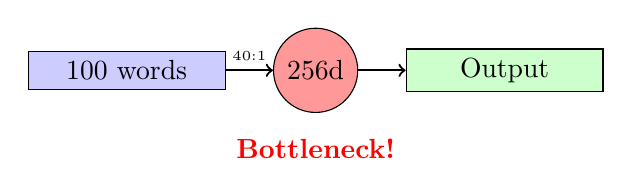
\begin{tikzpicture}[scale=0.6]
            \node[draw, rectangle, minimum width=2.5cm, fill=blue!20] (in) at (0,0) {100 words};
            \node[draw, circle, fill=red!40] (ctx) at (4,0) {256d};
            \node[draw, rectangle, minimum width=2.5cm, fill=green!20] (out) at (8,0) {Output};

            \draw[->, thick] (in) -- (ctx) node[midway, above] {\tiny 40:1};
            \draw[->, thick] (ctx) -- (out);

            \node[below of=ctx, node distance=1cm, text=red] {\textbf{Bottleneck!}};
        \end{tikzpicture}
        \end{center}

        \textbf{Results:}
        \begin{itemize}
            \item Short sentences: BLEU 31
            \item Long sentences: BLEU 8
            \item 74 percent quality drop!
        \end{itemize}

        \column{0.48\textwidth}
        \textbf{WITH Attention:}
        \begin{itemize}
            \item Keep all encoder states
            \item Dynamic context each step
            \item Minimal information loss
        \end{itemize}

        \begin{center}
        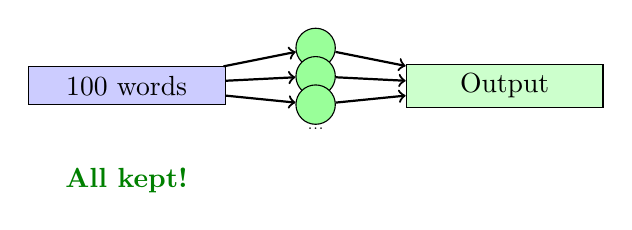
\begin{tikzpicture}[scale=0.6]
            \node[draw, rectangle, minimum width=2.5cm, fill=blue!20] (in) at (0,0) {100 words};

            \node[draw, circle, fill=green!40, minimum size=0.5cm] (ctx1) at (4,0.8) {};
            \node[draw, circle, fill=green!40, minimum size=0.5cm] (ctx2) at (4,0.2) {};
            \node[draw, circle, fill=green!40, minimum size=0.5cm] (ctx3) at (4,-0.4) {};
            \node at (4,-0.9) {\tiny ...};

            \node[draw, rectangle, minimum width=2.5cm, fill=green!20] (out) at (8,0) {Output};

            \draw[->, thick] (in) -- (ctx1);
            \draw[->, thick] (in) -- (ctx2);
            \draw[->, thick] (in) -- (ctx3);

            \draw[->, thick] (ctx1) -- (out);
            \draw[->, thick] (ctx2) -- (out);
            \draw[->, thick] (ctx3) -- (out);

            \node[below of=in, node distance=1.2cm, text=green!50!black] {\textbf{All kept!}};
        \end{tikzpicture}
        \end{center}

        \textbf{Results:}
        \begin{itemize}
            \item Short sentences: BLEU 33 (+2)
            \item Long sentences: BLEU 24 (+16!)
            \item Only 27 percent drop
        \end{itemize}
    \end{columns}

    \vspace{0.5em}
    \begin{tcolorbox}[colback=green!10!white,colframe=green!75!black]
    \textbf{Impact:} Attention improves long-sentence quality by \highlight{300 percent}!
    \end{tcolorbox}
\end{frame}

\begin{frame}[t]{Visualizing Attention: What the Model Learns}
    \textbf{Attention weights reveal learned alignments:}

    \vspace{0.5em}
    \begin{center}
    \includegraphics[width=0.7\textwidth]{../figures/week4_attention_heatmap.pdf}
    \end{center}

    \vspace{0.5em}
    \textbf{Key observations:}
    \begin{itemize}
        \item Diagonal patterns = similar word order
        \item Off-diagonal = word reordering (e.g., adjective position)
        \item Multiple focus points = phrases translate to multiple words
        \item \highlight{Model discovers alignment without explicit supervision!}
    \end{itemize}

    \vspace{0.5em}
    \textbf{This is interpretability:} We can see what the model is ``thinking''
\end{frame}

\begin{frame}[t]{From Seq2Seq to Modern NLP}
    \textbf{The foundation you've learned:}

    \vspace{0.5em}
    \textbf{Core concepts (now clear to you):}
    \begin{enumerate}
        \item \textbf{Embeddings:} Words as vectors (numerical meaning)
        \item \textbf{Hidden states:} Evolving understanding
        \item \textbf{Encoder-Decoder:} Separate reading from writing
        \item \textbf{Context vectors:} Compressed representation
        \item \textbf{Attention:} Selective focus to avoid bottleneck
    \end{enumerate}

    \vspace{0.5em}
    \textbf{How this evolved into modern AI:}

    \begin{center}
    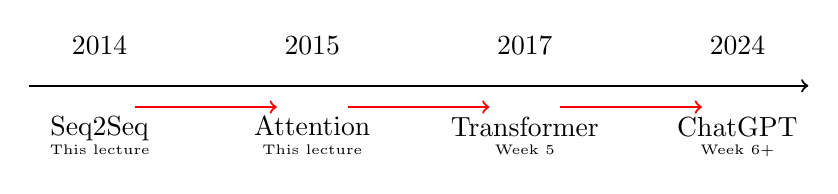
\begin{tikzpicture}[scale=0.9]
        \draw[->, thick] (0,0) -- (11,0);

        \node[above] at (1,0.3) {2014};
        \node[below] at (1,-0.3) {Seq2Seq};
        \node[below] at (1,-0.7) {\tiny This lecture};

        \node[above] at (4,0.3) {2015};
        \node[below] at (4,-0.3) {Attention};
        \node[below] at (4,-0.7) {\tiny This lecture};

        \node[above] at (7,0.3) {2017};
        \node[below] at (7,-0.3) {Transformer};
        \node[below] at (7,-0.7) {\tiny Week 5};

        \node[above] at (10,0.3) {2024};
        \node[below] at (10,-0.3) {ChatGPT};
        \node[below] at (10,-0.7) {\tiny Week 6+};

        \draw[->, thick, red] (1.5,-0.3) -- (3.5,-0.3);
        \draw[->, thick, red] (4.5,-0.3) -- (6.5,-0.3);
        \draw[->, thick, red] (7.5,-0.3) -- (9.5,-0.3);
    \end{tikzpicture}
    \end{center}

    \vspace{0.5em}
    \textbf{What's next (Week 5):}
    \begin{itemize}
        \item Transformer = ``What if we ONLY use attention, remove RNNs entirely?''
        \item Self-attention = Apply attention to input itself
        \item This enables: BERT, GPT, ChatGPT, Claude, and all modern LLMs
    \end{itemize}
\end{frame}

\begin{frame}[t]{Summary: The Complete Journey}
    \textbf{What you now understand from first principles:}

    \vspace{0.5em}
    \begin{enumerate}
        \item \textbf{Why embeddings:} Computers need numbers, embeddings give numerical meaning
        \item \textbf{Why hidden states:} Capture evolving understanding as we process sequences
        \item \textbf{Why encoder-decoder:} Separate reading (comprehension) from writing (generation)
        \item \textbf{Why context vectors:} Compress meaning, but creates bottleneck
        \item \textbf{Why attention:} Solve bottleneck by keeping all states and selectively focusing
        \item \textbf{Why dot product:} Geometric measure of relevance (vector alignment)
    \end{enumerate}

    \vspace{0.5em}
    \textbf{Technical terms you can now explain:}
    \begin{itemize}
        \item Word embedding, hidden state, context vector
        \item Encoder, decoder, seq2seq architecture
        \item Attention mechanism, attention weights
        \item Information bottleneck, compression ratio
        \item Dot product similarity
    \end{itemize}

    \vspace{0.5em}
    \textbf{Next week:} Remove the encoder/decoder RNNs, keep only attention = Transformers!
\end{frame}

\end{document}